\clearpage
\section{Monte Carlo methods}

\subsection{Monte Carlo simulation}
\begin{itemize}
	\item {\bf Goal:} Analyze complicated distributions by drawing samples from them: $P(\theta) \mapsto \{\theta^{(s)}\}$. Empirical statistics about the samples will approximate the true statistics of the distribution in question.
	\item {\bf Challenge:} From the vast majority of distributions, we don't know how to draw samples efficiently.
	\item {\bf Method:} 
	\begin{enumerate}
		\item Draw samples from an easy-to-sample distribution. ($P(a)$ in the figure below.)
		\item Transform the drawn values $\{a^{(s)}\}$ so they become samples from the distribution of question $\{\theta^{(s)}\}$.
	\end{enumerate}
\end{itemize}
\begin{figure}[h]
\centering
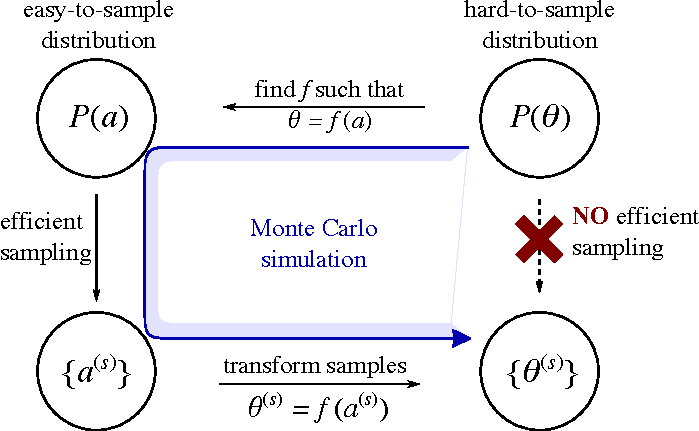
\includegraphics[width=0.5\textwidth]{./figs/07-MC.pdf}
\end{figure}


\no {\bf Example:} What is the distribution of the ratios of two normal variables?
\begin{itemize}
	\item Input: Two variables, $x_1$, $x_2$, we sample from standard normal distributions, $P(x_i) = \text{Normal}(x_i\;|\;0, 1)$.
	\item Output: We calculate the ratio, $y := x_1 / x_2$, the distribution of which is in question, i.e. $P(y) = \;?$
	\item MC method:
\begin{lstlisting}[language=python]
from scipy.stats import norm

samples = 1000
X1 = norm.rvs(loc=0, scale=1, size=samples)
X2 = norm.rvs(loc=0, scale=1, size=samples)
Y = X1 / X2
\end{lstlisting}

\end{itemize}

\begin{figure}[h]
\centering
	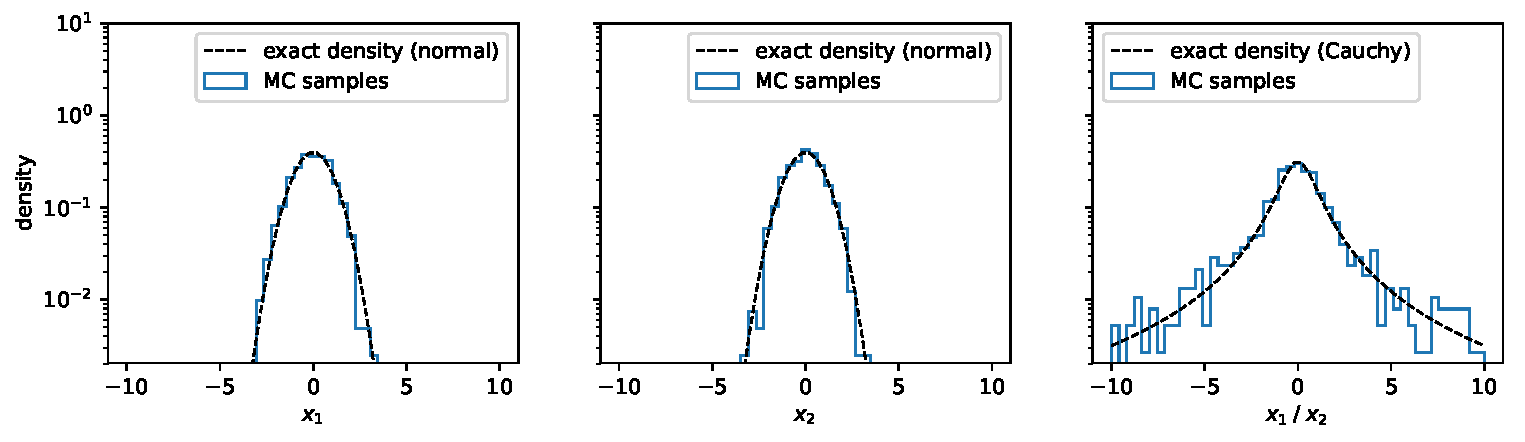
\includegraphics[width=0.95\textwidth]{./figs/07-Cauchy.pdf}
\end{figure}

\newpage
\no {\bf Example:} How is entropy of 3-categorical distributions from flat Dirichlet distributed?
\begin{itemize}
	\item Input: Parameter of 3-categorical distribution is $p = (p_1, p_2, p_3) \in [0,1]^{\times 3}$, such that $\sum_{k=1}^3 p_k = 1$. We sample this from a flat Dirichlet distribution, $P(p) = \text{Dirichlet}(p\;|\;\alpha = (1,1,1))$.
	\item Output: The entropy of a particular 3-categorical distribution with parameter $p$ is $h := H(p) = -\sum_k p_k \log_2 p_k$. We wish to determine the distribution of $h$, i.e. $P(h) = \;?$
	\item MC method:
\begin{lstlisting}[language=python]
import numpy as np
from scipy.stats import dirichlet

def entropy(p):
    h = 0
    for pk in p:
        if pk > 0:
            h += - pk * np.log2(pk)
    return h

alpha = (1,1,1)
samples = 10_000
p_samples = dirichlet.rvs(alpha, size=samples)
h_samples = []    
for p in p_samples:
    h_samples.append(entropy(p))
\end{lstlisting}

\item As the we simulate more Monte Carlo samples, the histogram or empirical density becomes smoother.
\end{itemize}

\begin{figure}[h]
\centering
	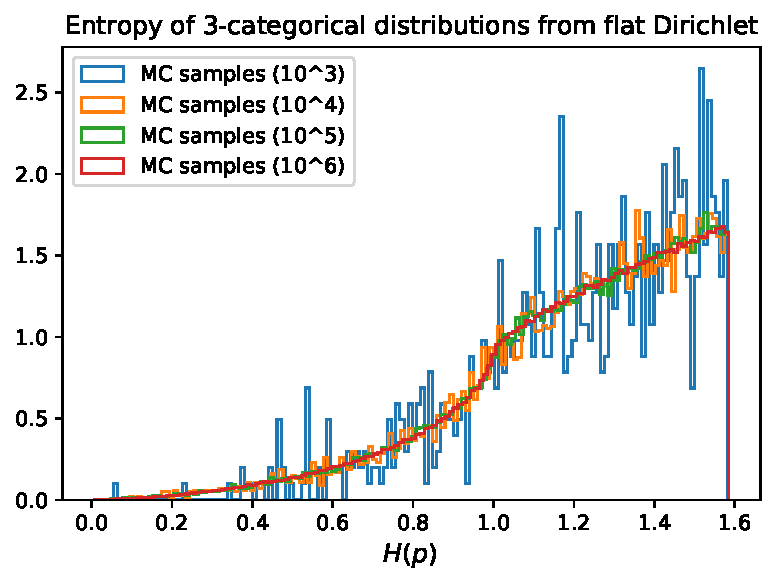
\includegraphics[width=0.7\textwidth]{./figs/07-entropy.pdf}
\end{figure}

\newpage
\no {\bf Example:} Monty Hall problem
\begin{itemize}
	\item Input: 
		\begin{itemize}
			\item In a game show, there a three doors $D = \{1,2,3\}$
			\item A reward is placed behind door $r\in D$ uniformly randomly, i.e. $P(r) = 1/3$ for all $r$.
			\item The player picks a door $p_1 \in D$ (``first pick'') uniformly randomly, i.e. $P(p_1) = 1/3$ for all $p_1$. (He doesn't know where the reward is.)
			\item The game show master (who knows where the reward is), picks a door from the remaining two that does not have the reward, and opens it, $o \in D_\text{can open}$, where $D_\text{can open} = D \setminus (\{r\} \cup \{p_1\})$ uniformly randomly, i.e. $P(o) = 1/ |D_\text{can open}|$, where $D_\text{can open} = 2$ if $r = p_1$, and $1$ if $r\neq p_1$.
			\item The game show master offers the player another chance to pick one of the remaining two doors $D_\text{remaining} = D \setminus \{o\}$. He can stick to his first choice, i.e. $p_2 = p_1$, or switch to the other door, i.e. $p_2 \in D_\text{remaining}\setminus \{p_1\}$
			\item The game show master opens door $p_2$, and the player wins if $p_2 = r$, and loses otherwise.
		\end{itemize}
	\item Output: What's the probability of winning with and without switching, i.e.
	\ba
		P(\text{win}\;|\;\text{switch}) = P(r=p_2\;|\;p_2 \neq p_1) &=& ?  \\
		P(\text{win}\;|\;\text{don't switch}) = P(r=p_2\;|\;p_2 = p_1) &=& ?
	\ea
	\item We can transcribe the relations between $r, p_1, o$ and $p_2$ directly to code and simulate 1000 games:
\begin{lstlisting}[language=python]
from numpy.random import choice

doors = {1, 2, 3}

games = 1000
wins_with_switch = 0
wins_with_no_switch = 0
for g in range(games):
    reward = choice(list(doors))
    pick_1 = choice(list(doors))

    can_open = doors - set([pick_1]).union(set([reward]))
    openned = choice(list(can_open))
    remaining = doors - set([openned])
    
    pick_2 = list(remaining - set([pick_1]))[0]
    if pick_2 == reward:
        wins_with_switch += 1
    
    pick_2 = pick_1
    if pick_2 == reward:
        wins_with_no_switch += 1
        
P_win_with_switch = wins_with_switch / float(games)
P_win_with_no_switch = wins_with_no_switch / float(games)
\end{lstlisting}
Yielding something similar to $P(\text{win}\;|\;\text{switch}) \approx 0.653$, and $P(\text{win}\;|\;\text{don't switch}) \approx 0.347$.

\end{itemize}

\subsection{Markov Chain Monte Carlo method}
For many real-world distributions $P(\theta)$, not only that a direct sampling method is unknown, but we do not even know a transformation to an easy-to-sample distribution. For such cases, Markov Chain Monte Carlo (MCMC) methods can be used to perform \emph{approximate} sampling. The most common use case of MCMC method is drawing samples from an unnormalized posterior.
\begin{itemize}
	\item {\bf Goal:} Draw samples from an unnormalized posterior (or ``target'' distribution) $P\s(\theta) \mapsto \{\theta^{(s)}\}$
	\item {\bf Challenge:} We don't know how to do this directly, or even indirectly via transformations.
	\item {\bf Method:} Generate a chain of variables $\theta^{0}, \theta^{1}, \ldots $, where each value is drawn by taking the previous value and the unnormalized posterior into account.
	\begin{enumerate}
		\item Choose a plausible $\theta^{(0)}$.
		\item Obtain a new $\theta^{(s+1)}$ value using the current value $\theta^{(s)}$ and the $P\s(\theta)$ function.
		\item Add the new value to the list of samples $\{\theta^{(s)}\}$. Return to step 2 with $s \leftarrow s+1$.
	\end{enumerate}
\end{itemize}
\begin{figure}[h]
\centering
	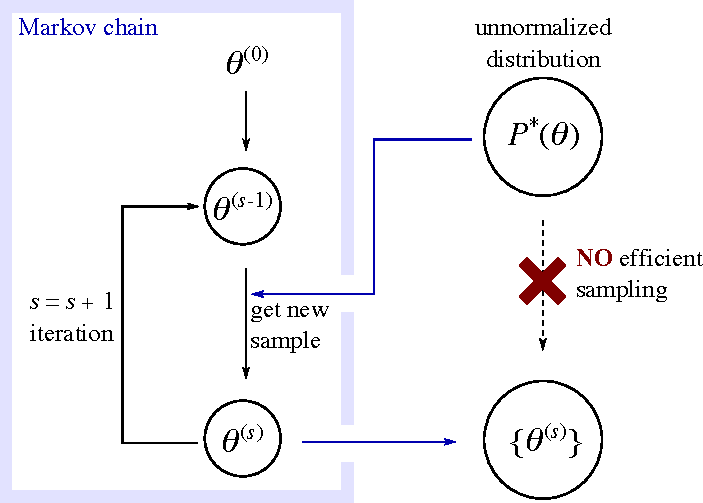
\includegraphics[width=0.5\textwidth]{./figs/07-MCMC.pdf}
\end{figure}
Several different Markov chain-based methods exist, which differ in how they combine the previous sample and the target distribution to draw a new sample: Metropolis-Hastings sampling, Gibbs sampling, Hamiltonian sampling, and more. They differ

\subsection{Metropolis-Hastings sampling}
In each iteration, the Metropolis-Hastings method proposes a random move $\theta^{(s)} \mapsto \theta^\text{new}$, which is eventually accepted or rejected based on how well it complies with the target distribution $P\s(\theta)$. The most common version (for sampling unbound variables) uses a normal distribution for generating proposals:
\begin{enumerate}
	\item Start with a plausible $\theta^{(0)}$.
	\item Propose a new value: $\theta^\text{new} = \theta^{(s)} + \varepsilon$, where $\varepsilon$ is drawn from $P(\varepsilon) = \text{Normal}(\varepsilon\;|\;0, \sigma^2)$, where $\sigma$ is the fixed ``typical step size'' (the value of which often needs careful choosing).
	\item Evaluate the log probability improvement, $\Delta L = \log P\s(\theta^\text{new}) - \log P\s(\theta^{(s)})$, and depending on its value, we obtain $\theta^{(s+1)}$:
	\begin{enumerate}
		\item If $\Delta L \geq 0$, then 
		\be	
			\theta^{(s+1)} = \theta^\text{new},
		\ee
		\item if $\Delta L < 0$, then 
		\be
			\theta^{(s+1)} = 
			\left\{
			\begin{array}{ll}
				\theta^\text{new}& \text{with probability } \exp(\Delta L)
				\\
				\theta^{(s)} & \text{with probability } 1 - \exp(\Delta L)
			\end{array}
			\right.
		\ee
	\end{enumerate}

\newpage
\no {\bf Example:} A one-dimensional, bimodal distribution
\begin{itemize}
	\item Unnormalized distribution: $\log P\s(x) = x / 2 - \big(1 - x^2\big)^2$, where $x \in \mathds{R}$.
	\item 1-dimensional Metropolis-Hastings sampler:
\begin{lstlisting}[language=python]
def propose_MH(x, stepsize):
    epsilon = norm.rvs(loc=0, scale=stepsize)
    return x + epsilon

def new_sample_MH(x_current, x_proposed, log_Pstar):
    delta_L = log_Pstar(x_proposed) - log_Pstar(x_current)
    if delta_L >= 0:
        return x_proposed
    if np.random.random() < np.exp(delta_L):
        return x_proposed
    else:
        return x_current
\end{lstlisting}
	\item Applying it to the $\log P\s$ in question:
\begin{lstlisting}[language=python]
def log_Pstar_camel(x):
    return 0.5 * x -(1 - x**2)**2

x0 = 0
stepsize = 0.1
iterations = 20000
x_samples = []

x_curr = x0
for it in range(iterations):
    x_proposed = propose_MH(x_curr, stepsize)
    x = new_sample_MH(x_curr, x_proposed, log_Pstar_camel)
    x_samples.append(x)
    x_curr = x
\end{lstlisting}
\end{itemize}

\begin{figure}[h]
\centering
	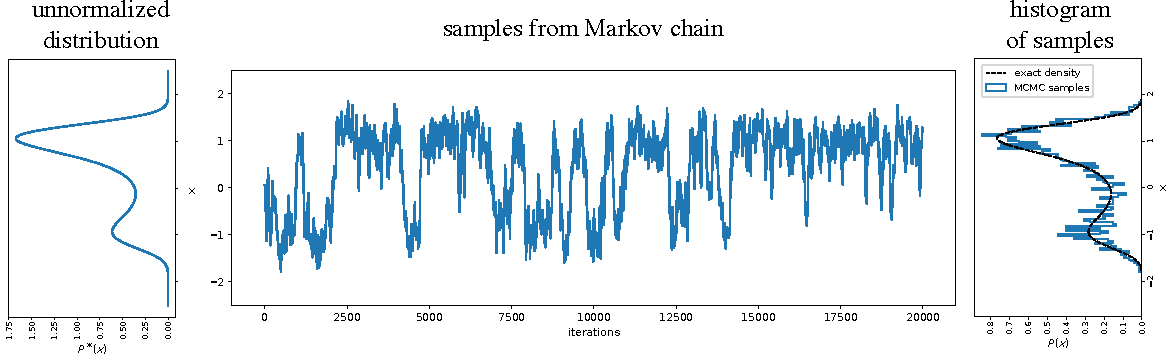
\includegraphics[width=1.1\textwidth]{./figs/07-camel-MH.pdf}
\end{figure}
\end{enumerate}





